\part{Iterative Methods}

\chapter{Overview of Iterative Methods} 
 
With this lecture the flavor of the book changes. We move from direct methods, a classical topic that is rather thoroughly understood, to the relatively untamed territory of iterative methods. These are the methods that seem likely to dominate the large-scale computations of the future.

\section{Why iterate?}

\begin{itemize}
    \item Noniterative or ``direct'' algorithms require $ O(m^3) $ work. 
    \item Iterative methods can solve matrix problems in $ O(m^{2} ) $ operations.
\end{itemize}
 
\section{Structure, Sparsity, and Black Boxes}
\begin{itemize}
    \item Large matrix problems are far from random and they might have sparsity or structure. 
    \item The iterative algorithm requires nothing more thant the ability to determine $ Ax $ for any $ x $, which can make use of the sparsity. 
    \item Gaussian or Householder triangularization will destroy the sparsity. 
\end{itemize} 

\section{Projection into Krylov Subspaces}
 
 %────────────────────────────────────────
 \begin{definition}
 [Krylov subspaces]
 \label{def: Krylov subspaces}
 Given $ A\in \RR^{n \times n}, b\in \RR^{n} $, the associated Krylov sequence is
 \[
    b, Ab, A^{2} b, A^{3}b,\ldots 
 \]
 The corresponding Krylov subspaces are the spaces $ \{\langle b, Ab, A^{2} b,\ldots ,A^{m}b \rangle \}_{m=1}^\infty  $. 
 \end{definition}
 %────────────────────────────────────────
 
 The algorithms we shall discuss can be arranged in the following table: 

%────────────────────────────────────────
\begin{figure}[H]
    \centering
    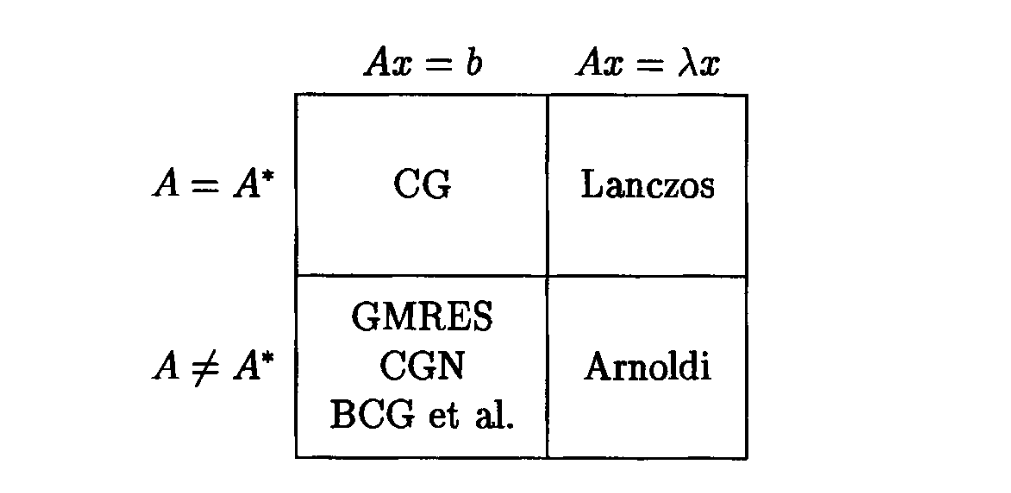
\includegraphics[width=0.5\textwidth]{figures/32-1.png}
\end{figure}
%────────────────────────────────────────
 
 \section{Works and Preconditioning}
 \begin{itemize}
    \item Gaussian elimination, QR factorization, and most other algorithms of dense linear algebra fit the following pattern: there are $O(m)$ steps, each requiring $O\left(m^2\right)$ work, for a total work estimate of $O\left(m^3\right)$. 
    \item The ideal iterative method in linear algebra reduces the number of steps from $m$ to $O(1)$ and the work per step from $O\left(m^2\right)$ to $O(m)$, reducing the total work from $O\left(m^3\right)$ to $O(m)$. Such extraordinary speedups do occur in practical problems, but a more typical improvement is perhaps from $O\left(m^3\right)$ to $O\left(m^2\right)$.
 \end{itemize} 
  
 \section{Direct Methods that Beat $ O(m^{3}) $}

  Finally, we must mention that there exist direct algorithms-finite, in principle exact-that solve $A x=b$ and related problems in less than $O\left(m^3\right)$ operations. The first algorithm of this kind was discovered in 1969 by Volker Strassen, who reduced Gauss's exponent of 3 to $\log _2(7) \approx 2.81$, and subsequent improvements have reduced the best known exponent to its current value of $\approx 2.376$ due to Coppersmith and Winograd. The history of these best known exponents is recorded in Figure 31.1.

  %────────────────────────────────────────
  \begin{figure}[H]
    \centering
    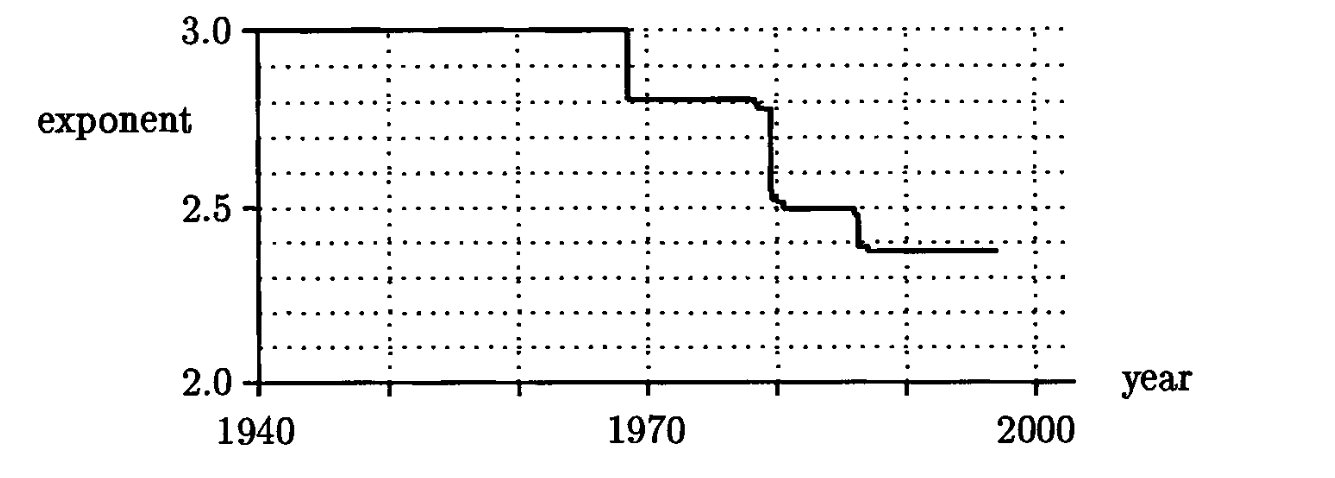
\includegraphics[width=0.8\textwidth]{figures/32-2.png}
    \caption{Best known exponents for direct solution of $ Ax=b $ for $ m\times m $ matrices, as a function of time. Until 1968, the best known algorithms were of complexity $ O(m^3) $. The current best known algorithm solves $ Ax=b $ in $ O(m^{2.376}) $ flops, but the constants are so large that this algorithm is impractical. }
  \end{figure}
  %────────────────────────────────────────